The board design has been made in \textit{KiCAD}. \textit{Git} was used for version control. In the schematics (Appendix \ref{append:power}) one can see that the whole board consists of three main building blocks: Connectors, a LED driver with feedback and two step-down converters. A part of the LED driver is also "abused" to drive the OLED. 
\subsection{Microcontroller Power Supply}
It is the LM2840 which in combination with a simple voltage divider ensures the 2.8 V for Vcc. All step-down converters use the same inductor with a value of 33 uH. It is a low-cost, quite small, shielded inductor which is ment to be used for switching power supplies. Moreover all step-down converters are enhanced with a SMD schottky diode and a of course at least one SMD capacitor for smoothing the output signal. As it is good practice to do so all ICs are making use of decoupling capacitors. 
\subsection{Designated USB Charging Port}
For charging ones phone the TS30012, another step-down converter IC, is used. The feedback voltage divider of this IC is already integrated and does not need to be provided externally as the IC provides fixed 5 V output. The output is connected to a USB connector type A. This IC can deliver up to 2 A. An interesting feature of the phone charging circuitry on the power board is the "Dedicated Charging Port" (DCP) functionality. The TPS2514 is a small, easy-to-use, 6-pin component, which complies to the USB standard and a majority of the minefield of propriatary standards to signal a DCP. Now you might ask: What does this mean? Well this means, that if you connect your IPhone, it will know, that it can draw more than 100 mA, which is the minimum current provided by a normal USB 2.0 port. Otherwise the current drawn by the phone will be limited. The charging functionality can be turned on and off via a GPIO pin. The TS30012 comes in a QFN16 package (pad pitch of 0.5 mm) to save space.   
\subsection{HW Debugging}
For testing purposes a lot of test points have been included into the design. Futhermore there are LEDs for different voltages (e.g. Vcc).
\subsection{RGB LED Driver}
The LED driver consists of an actual power electronics part and a feedback part. The main idea is, that the current driven through the three color channels of the RGB LED (see fig. \ref{fig:led}) can be controlled by software (PID controller). In the power electronics part there are three analog circuits. Each circuit mainly consists of a p-channel MOSFET, which is switched by a NPN bipolar transistor. This bipolar transistor gets its intput signal from the µProcessor (PWM). By pulling the 20 V to GND the PMOS "sees" a negative gate-to-source voltage and opens. The additional bipolar transistor ensures, that the gate-source capacity is charged fastly as soon as the PWM NPN blocks. In this case the base is pulled up via \SI{10}{\kilo\ohm} to 20 V and as long as the collector (which has the same potential as the gate of the PMOS) does not also have 20 V the NPN keeps pumping charges into the gate-source capacity. The simple silicon diode ensures that the gate-charging NPN has no effect as soon as the PWM NPN opens. The rest of the circuit is again a standard step-down converter. At the output of every single color channel power circuit one can see a shunt resistor of \SI{0.1}{\ohm}. This shunt resistor is combined with a simple low-pass filter. The feedback signal is amplified by a differential amplifier which comes after the filter. The signal is supposed to be between 0 V and 1 V (if the internal reference voltage is used). By doing so one can use all bits of the ADC and therefore supress quantization noise. 
\newpar
So as there are three color channels (red, green and blue) one needs three operational amplifiers. Hence the LM324QT, which provides four operational amplifiers, has been chosen. Of course the decision has been made to take QFN16 packaging once more to save even more space. An additional operational amplifier was now ready to be used as a digital-analog converter to drive the OLED screen (this was referred to earlier as "abuse"). For this reason a low-pass filter is attached to the input of the fourth opamp. Apart from that the opamp is configured just like a standard non-inverting amplifier. By software the OLED screen brightness is steerable. The feedback from the OLED is generated by a voltage divider. 
\begin{figure}
	\centering
	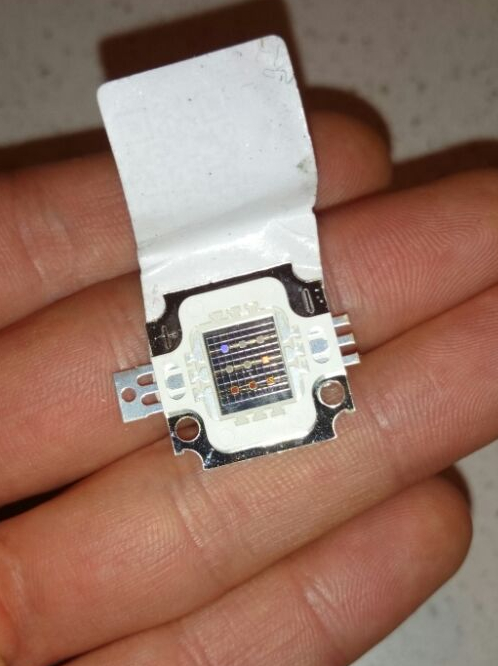
\includegraphics[width=0.3\textwidth]{./fig/led.jpg}
	\caption{10 W RGB LED}
	\label{fig:led}
\end{figure}                    
